\Gls{castor} is an open source fully quantitative reconstruction platform that has been developed within a collaboration platform, financed by France Life Imaging (FLI). This PhD project relied heavily on the use of \gls{castor} for developing and performing reconstructions, on both simulated and real patient data. The work conducted in this project resulted in the development and evaluation of new functionalities, which are now part of the released public version. These are described in detail in chapter~\ref{chap:Results_CASToR}. 

In this chapter we provide a short introduction into the functionalities and innovative reconstruction methods provided in \gls{castor} that play an important role for the work performed in this PhD project. 
The platform supports \gls{pet}, \gls{spect} and \gls{ct} imaging. 
In this short description the focus is on PET reconstruction for static and dynamic imaging. A more detailed description of all the functionalities of \gls{castor} can be found on the official website and the official publication by Merlin~\textit{et al.}\cite{Merlin2018}. 

The main philosophy behind the design of the platform is genericity and abstraction. The code architecture is divided into main components which manage global tasks. These are named as "managers" and handle tasks such as reading datafiles, handling reconstruction dynamic aspects, managing the scanner geometry, computing a projection, etc. 
Each "manager" component is utilising abstract classes which include a representation of all the desired functionalities, required by the component, as virtual functions. The final step is to implement these virtual functions using a specific implementation as a specific class. 
Using this strategy generic code of basic functionalities is implemented only once, while specific classes require coding of only the basic functionalities that are specific to the implementation. This allows for development of specific classes with minimal amount of coding, that can be used as plug-ins to the existing generic architecture. 
An example of this design is shown in figure~\ref{fig_2_4:oProjectorManager}, with the \textit{oProjectorManager} as the main component, the \textit{vProjector} as the virtual class which includes all the generic functionalities of a projector, and finally the projector implementations which include code that calculates a projection using a specific implementation. Template classes are also provided for instructing how new implementations, of projectors in this example, can be made. 

\begin{figure} [h!]
\centering
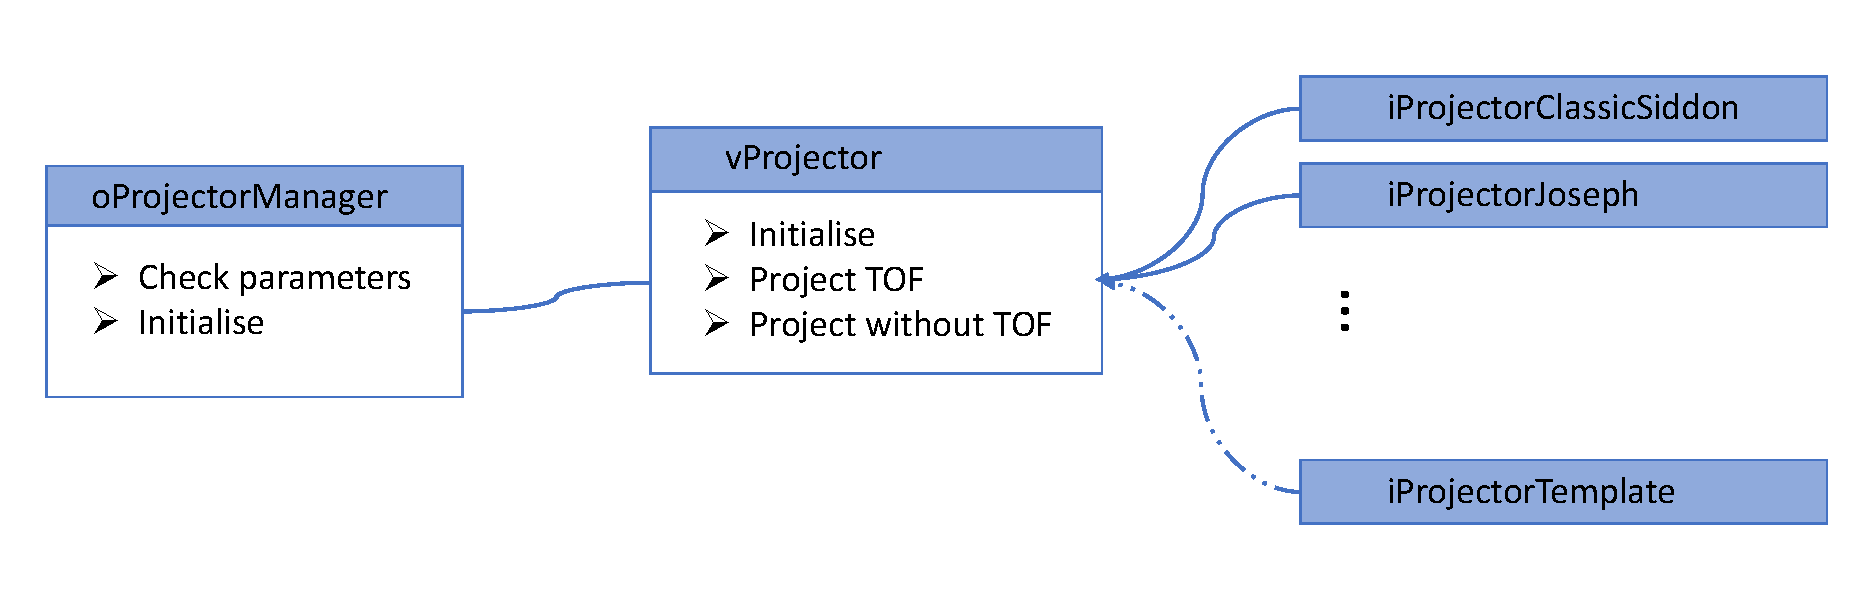
\includegraphics[scale=0.50,angle=0]{2_Theory_Methods/figures/oProjectorManager.pdf}
\caption{Example of \gls{castor} abstraction design for the projection component.} 
\label{fig_2_4:oProjectorManager}
\end{figure}


\section{Data}
Data are provided in \gls{castor} in the form of a \gls{castor} datafile, which is based on a generic data description that is similar for both list-mode and histogram data. 
The minimum information required for each event of the datafile are a time-stamp, pair of detector IDs and number of events(for histograms). Additional information can also be provided per event such as scatter and random corrections, normalisation factors, \gls{tof}, gating information, etc. 

List-mode data maintain the exact timing information of each event. This is advantageous in reconstruction of dynamic datasets, as the separation of the list-mode data the desired frames for reconstruction is made within \gls{castor}, during reconstruction and using the framing selected by input of reconstruction parameters. As such, list-mode datafiles allow for re-use of the data with multiple framing definitions without need of pre-process the data. 

Histograms are by definition events that have been histogrammed for a specific time range. All events of a \gls{castor} histogram datafile have the same timestamp which is the timestamp of the first time point of the histogrammed data. Thus dynamic data need to be pre-processed into individual histograms, one histogram per dynamic frame, using a predefined framing definition.
Multiple histograms from a dynamic dataset can be concatenated together into a single file, before used in \gls{castor} for reconstruction. In this case reconstructions can be performed using the concatenated file and solely with the framing definition used to created the histograms. 
Use of other framing definitions would require re-processing of the data before providing them into \gls{castor} for reconstruction.

In this project, when possible, use of list-mode datafiles was preferred due to the offered flexibility. 
List-mode datafiles were used for reconstructions of real PET datasets, while histograms were used for reconstructions of simulated datasets (from analytical simulations).

\section{Geometry}
A generic description of the geometry of an imaging system in \gls{castor} allows for the definition of any \gls{pet} system. Individual detector elements are defined by 3D Cartesian coordinates and an orientation vector. These are pre-computed and input as look-up-tables, or are computed by \gls{castor} using a system definition similar to that used for GATE simulations~\cite{Jan2011}.

In this project the geometries of the Signa PET/MR and Siemens mMR PET/MR scanners were used, for which lookup tables are provided with the current version of \gls{castor} (Version 3.1). 

\section{Dynamic aspects}

The use of generic functions and generic datafile definition allows for the reconstruction to be performed by a single implementation of an iterative algorithm. The main steps performed within this iterative algorithm are shown in algorithm~\ref{algo:CASToR_Core}. 

The platform is designed to handle three temporal levels of binning. It makes temporal binning for dynamic frames and binning in two levels of gating (for cardiac and respiratory motions). Alternatively, one of the two levels of gating can be used for splitting the data for involuntary motion corrections. 

\begin{algorithm} [h!]
  \For{$i\leftarrow 1$ \KwTo nb of iterations}
  {
   \For{$j\leftarrow 1$ \KwTo nb of subsets}
   {
    \emph{index start}$\leftarrow$ current subset\;
    \emph{index step}$\leftarrow$ number of subsets\;
    Perform Image-based Convolution (forward step)\;
    \tcp{loop over bed positions}
    \For{$s\leftarrow 1$ \KwTo nb of beds}
    {
      \tcp{Parallel loop}\  
      \For{$e\leftarrow$ index start \KwTo nb events \KwStep index step}
      {
        \textbf{Get Event corresponding to }\emph{\textbf{e}}\;
        %Check Image (forward) Deformation for \emph{e}\;
        \If{Deformation required for $e$}{
        Perform Image-Based Deformation(forward step)\;}
        \tcp{apply axial offset for bed}
        \textbf{Apply bed offset}\;
        \tcp{Recover system matrix elements associated with this event}
        \textbf{Compute/load the system matrix elements associated to this Event}\;
        \tcp{Compute the update term associated to the optimization algorithm}
        \textbf{Compute the forward model}\;
        \textbf{Compute the update term(s) to be back-projected}\;
        \textbf{Back-project update term(s)}\;
      }
    }
    %\textbf{Synchronize all data}\;
    Perform Image-based Convolution (backward step)\;
    Perform Image-Based Deformation (backward step)\;
    \textbf{Update image according to the optimization algorithm}\;
    \tcp{Make use of a dynamic model with nested optimisation}
    \If{Nested use of Dynamic model}{
    Estimate/Fit dynamic model \;
    Estimate image from fitted dynamic model \;
    }
   }
  }
\caption{CASToR core iterative loop}
\label{algo:CASToR_Core}
\end{algorithm}

\subsection{Motion correction and image deformation}
Image based deformations can be performed within the iterative loop, over gate bins or bins defined by involuntary motion, that can counteract effects of motion in the data and result in motion free reconstruction using all data (without need of rejection or individual reconstructions per gate).
Unfortunately, with the current version of \gls{castor} the available implemented deformations are limited to rigid deformation.
Although this deformation can be adequate for brain imaging, it is not suitable for modeling elastic motion that is commonly found in whole body studies. Owing to this limitation at this time, no motion correction was considered in the reconstructions and evaluations performed in this project.

\subsection{Dynamic reconstruction}
Multi-frame reconstruction of individual frames can be performed within \gls{castor} with a single execution. The framing is provided in the reconstruction input. For each event a dynamic switch function is used to identify to which frame the data belongs to. Image update is performed accordingly to each respective frame image.

The dynamic series of images is stored in \gls{castor} using a set of basis functions and images of basis coefficients, as described before in equation~\ref{eqn:2_3_LinearBasis}. 
In the case of individual frame reconstructions, the set of basis is a identity matrix and the coefficient images are the frame images. 

For dynamic reconstructions using a dynamic model, the model derived basis functions can be used directly in \gls{castor}, in which case the image update terms directly update the parametric images.
As discussed previously in~\autoref{section:Fully_4D_reconstruction}, dynamic reconstruction can be performed efficiently when using optimisation transfer principles and nested optimisation for the dynamic model fitting. 
To perform this in \gls{castor} a new component was created (named \textit{oDynamicModelManager}) to handle preparation and fitting of dynamic models. The component and its accompanying abstract and specific classes were developed and tested as part of this project, in collaboration and with guidance by this project participants and Dr Thibaut Merlin.
The developments are described in detail in the !Results! 
\todo[inline,size=\Large, color=red!40]{Add reference details here after written results!}

\subsection{Multi-bed reconstruction}

With the generic description of the geometry implemented in CASToR, system matrix elements related to each detection event are computed on-the-fly, by projecting a ray though image space, or they are read from a pre-computed system matrix. 
The on-the-fly computation allow for additional flexibility, which has been used to enable direct multi-bed reconstruction. 
As described in section~\ref{WB_Static_SS}, multi-bed Step and Shoot (SS) acquisitions make use of overlapping beds to increase the sensitivity at the edges of each bed's FOV. This the raw PET data for a static WB acquisition comprise of a number of acquisition datasets, one for each bed position. We can define the WB raw PET dataset as the collection

\begin{equation}
   \bm{y} = \Big\{ {\bm{y}_s,s=1,...,n_s} \Big\} \\ , \\
\end{equation}
where
\begin{equation}
   \bm{y_s} = \Big\{ {y_{si},i=1,...,n_i} \Big\} \\ , \\
\end{equation}

with $s$ being the index of the $n_s$ number of axial bed positions.

By incorporating the offset of each bed position in the projection operation, equation~\ref{eqn:MLEM} can be re-written for direct reconstruction of the whole acquisition effective \gls{fov}, using all acquired raw data, as
\begin{equation}
\lambda_j^{(k+1)} = \frac{\lambda_j^{(k)}}{\sum_{s=1}^{n_s} \sum_{i=1}^{n_i} P_{sij}} 
\sum_{s=1}^{n_s} \sum_{i=1}^{n_i} P_{sij} 
\frac{y_{si}}{\sum_{d=1}^{n_j} P_{sid}\lambda_d^{(k)} + B_{si} } \\ , \\
\label{eqn:MLEM}
\end{equation} 

where now the image estimate $\lambda_j^{(k)}$ has the dimensions of the whole effective \gls{fov}, and the additive correction terms $B_{si}$ is provided for each respective bed position $s$. 

Direct reconstruction of multi-bed data, which combines data from overlapping acquisitions within the iterative reconstruction loop, improves the statistics of the overlapping region that are available for each iteration. It has been shown that this technique can result in improved contrast to noise ratios at the overlapping regions, for specific levels of acquisition statistics~\cite{Ross2004}. 

This method has been implemented in CASToR by making use of an additional loop over bed positions and an "Apply bed offset" function, which applies the bed offset to the projector for each bed, as seen in the CASToR iterative algorithm~\ref{algo:CASToR_Core}.
